\chapter{بررسی کارهای مرتبط}
\section{دسته‌بندی روش‌های موجود برای مسئله}
در طی چهار دهه گذشته روش‌های گوناگونی برای مسئله \gls{atm} پیشنهاد داده شده است.
با وجود این که هدف نهایی هر سیستم \gls{ATM} استخراج حالت نوشتاری موسیقی از روی
سیگنال‌های صوتی هست ولی اکثر راه‌حل‌های موجود تلاش می‌کند با رسید به یک هدف
میانی مسئله را حل کنند. با توجه به ماهیت این هدف‌های میانی و ساختار آن‌ها
می‌توان این روش‌ها را به چهار دسته کلی تقسیم کرد:
\begin{itemize}
    \item در سطح فرم
    \item در سطح نت
    \item در سطح جریان
    \item در سطح نماد
\end{itemize}

آوانویسی در سطح فرم یا \gls{mpe}، تخمین تعداد و \gls{pitch} نت‌های موجود در هر
یک فرم زمانی است. این فرم‌ها معمولا طولی در حدود چند میلی ثانیه دارند. هرچند این
تخمین معمولا برای هر فرم به صورت جدا انجام می‌شود ولی اطلاعات زمینه‌ای معمولا در
یک مرحله‌ پس‌پردازیش برای روی نتیجه به دست آمده اعمال می‌شوند تا دقت را افزایش
دهند. روش‌هایی که در سطح فرم تلاش می‌کنند که آوانسی را انجام دهند از مفهوم نت
استفاده‌ای نمی‌کنند و معمولا با هیچ فهموم موسیقیایی درگیر نمی‌شود.

حجم زیادی از روش‌های موجود در سطح فرم کار می‌کنند. روش‌هایی مانند پردازش سیگنال
به صورت سنتی \cite{emiya2009multipitch,su2015combining}، مدل‌های برپایه احتمال
\cite{duan2010multiple}، روش‌های برپایه بیز \cite{peeling2009generative}، \gls{nmf}
\cite{smaragdis2003non,vincent2009adaptive,benetos2013automatic,fuentes2013harmonic}
و روش‌های برپایه \gls{nn} \cite{sigtia2016end,kelz2016potential}. تمام این
روش‌ها نقاط قوت و ضعف خود را دارند و هنوز روشی به عنوان روش واحد انتخاب نشده
است. برای مثال روش‌های بر پایه پردازش سیگنال ساده‌تر و سریع‌تر هستند و قابلیت
تعمیم بالاتری به سازهای مختلف دارند. در حالی که روش‌های بر پایه \gls{dl} بر روی
یک ساز خاص، مثلا پیانو، به نتایج بهتری دست یافته‌اند. روش‌های بیضی می‌توانند
مدل‌سازی کاملی از فرآیند تولید صوت ارائه دهند، در حالی که به شدت پیچیده‌تر و
کندتر هستند.

آوانویسی در سطح نت، یک مرحله از \gls{MPE} سطح بالاتر هست از این جهت که این
روش‌ها فقط وجود یا عدم وجود نت در یک فرم را بررسی نمی‌کنند، بلکه فرم‌ها را به هم
وصل کرده و نت‌ها را در طول زمان بررسی می‌کنند. در \gls{ATM} معمولا هر نت را با
سه ویژگی \gls{pitch}، onset و offset مشخص می‌کنند \cite{klapuri2007signal}. با
توجه مبهم بودن offset در نت، در بعضی از سیستم‌ها، معمولا در نظر گرفته نمی‌شود.
در نتیجه مدل فقط \gls{pitch} و onset را پیشبینی می‌کنند.

حجم زیادی از روش‌های در سطح نت معمولا پس‌پردازیش‌هایی بر روی خروجی یک سیستم
\gls{MPE} هستند. به عنوان روش‌های استفاده شده می‌توان از \gls{hmm}
\cite{nam2011classification} و \gls{nn} \cite{boulanger2012modeling} نام برد. در
پس‌پردازیش‌های انجام شده معمولا هر نمونه به صورت جدا بررسی می‌شود و رابطه بین
نت‌ها همزمان در نظر گرفته نمی‌شود که باعث تشخیص اضافه یا کمتر نت‌هایی می‌شود که
هارمونیک مشترک با نت‌های درست دارند. از این جهت روش‌هایی بر پایه مدل موسیقی
پیشنهاد شده است تا در ارتباط بین نت‌ها نیز در نظر گرفته شود
\cite{boulanger2012modeling, sigtia2016end}. بخش دیگری از روش‌ها نت‌ها را مستقیم
از روی سیگنال صوت استخراج می‌کنند. برخی دیگر ابتدا onset هر نت را پیدا می‌کنند و
سپس \gls{pitch} را بین آن‌ها تشخیص می‌دهند \cite{marolt2004connectionist}. برخی
دیگر حتی کل اطلاعات را با هم استخراج می‌کنند
\cite{cogliati2016context,ewert2016piano,hawthorne2017onsets}.

آوانویسی در سطح جریان یا \gls{mps} هدفش گروه بندی نت‌ها تخمین زده شده در
مجموعه‌ای جریان هست که هر جریان معمولا متناظر با یک ساز هست. این گروه از روش‌ها
ارتباط نزدیکی با \gls{iss} دارد. یکی از مزایای \gls{MPS} نسب به روش‌های قبلی
بررسی و تاثیر دادن \gls{timber} است. کارهای انجام شده در این سطح بسیار محدود
هستند.

تمام سه روش توضیح داده شده خروجی اصطلاحا پارامتری دارند. علت این نامگذاری این
هست که این آوانویسی انجام شده، یکی از پارامترهایش سیگنال صوتی ورودی هست. این
آوانویسی‌ها با وجود این که تا حدی از مفاهیم مسیقیایی استفاده می‌کنند ولی خروجی
آن‌ها هنوز اختلاف زیادی با سطح مجردسازی انجام شده در \gls{sheet music} دارد.
مهمترین این اختلاف‌ها زمان هست که در هر سه روش در واحد ثانیه اندازه گرفته
می‌شود. در حالی که در موسیقی زمان در واحد ضرب اندازه گرفته می‌شود. همچنین
\gls{pitch} در فراکنس هست در حالی که در موسیقی معمولا هر نت نامی مانند دو مینور
دارد و باتوجه به گام قطعه تعریف می‌شود. در نهایت مفاهیمی مانند میزان، ضرب آهنگ،
تمپو، گام و هارمونی کاملا حذف شده‌اند.

هدف آوانویسی در سطح نماد این هست که خروجی سیستم، نمادگذاری قابل لمس برای انسان
باشد که تمام اطلاعات موسیقیایی لازم را در بردارد. خروجی مانند \gls{sheet music}.
آوانویسی در این سطح نیاز به درک عمیق مفاهیم موسیقی مانند هارمونیک و ریتم دارد.
ساختارهای هارمونیک مانند گام و آکوردها باعث تغییر شکل نمایش \gls{pitch} می‌شوند.
ساختارهای ریتمیک مثل ضرب و میزان باعث می‌شود که طول نت‌ها از ثانیه مستقل شود.

چندین مطالعه تلاش کرده‌اند که ساختارهای موسیقیایی رو از روی سیگنال صوتی یا
\gls{MIDI} به دست آید انجام شده است. با این وجود مطالاعات خیلی کمی برای روی یک
سیستم آوانویسی کامل انجام شده است که از این مفاهیم استفاده کند.

با این وجود که روش‌های بسیار متفاوتی برای \gls{atm} وجود دارد ولی در دهه گذشته
بهترین دقت به دست آمده از دو خانواده از روش‌ها بوده است:
\begin{itemize}
    \item \gls{nmf}
    \item \gls{nn}
\end{itemize}
هر دو خانواده این مسائل برای مسائل بسیار متفاوتی مانند پردازش گفتار، پردازش
تصویر و سیستم‌های پیشنهاددهنده استفاده شده‌اند و نتایج بسیار رضایت بخشی به دست
آورده‌اند. در ادامه استفاده هر دو روش برای سیستم‌های \gls{ATM} بررسی می‌شود.

\section{روش‌های برپایه‌ی فاکتورگیری نامنفی ماتریس}

\section{روش‌های برپایه‌ی شبکه‌ عصبی}
همانند دیگر مسائل مرتبط با حوزه تشخیص الگو، شبکه‌های عصبی تاثیر قابل توجهی بر
روی مسئله \gls{atm} و به صورت کلی‌تر حوزه \gls{mir} داشته‌اند. \gls{nn} توانایی
یادگیری توابع غیرخطی پیچیده‌ را دارند که به آن‌ها برای حل مسائل کمک می‌کند. با
این وجود در مقایسه با حوزه‌ای مانند بینایی ماشین، سرعت رشد استفاده از \gls{nn}
برای حل مسئله \gls{atm} پایین بوده است. در ادامه تلاش می‌کنیم چند علت این موضوع
را بررسی کنیم.

یکی از اولین استفاده‌ها از \gls{nn} برای حل مسئله توسط
\cite{marolt2004connectionist} ارائه شده است. بخش اصلی این مدل استفاده از شبکه
تاخیر زمانی بوده است که همانند یک \gls{cnn} در بعد زمان عمل می‌کند. هر چند
انتشار این روش به ۲۰۰۱ برمی‌گردد ولی همچنان روشی موثر محسوب می‌شود و روش‌های
جدیدتر خود را با آن مقایسه می‌کنند.

یک روش نسبت جدیدتر \cite{bock2012polyphonic} استفاده از دو \gls{spec} به عنوان
ورودی است. یک از این \glspl{spec} دقت بالاتری در بعد زمان دارند که که برای تشخیص
شروع نت‌ها از آن استفاده می‌شود. \gls{spec} دیگر دقت بالایی در بعد فرکانس دارد.
از این دقت بالاتر برای تشخیص نت‌های با فراکنس پایین‌تر استفاده می‌شود. این
ورودی‌ها به یک شبکه چند لایه با ساتختار \gls{lstm} داده می‌شوند. این استفاده از
\gls{LSTM} دو مزیت دارد. اولین خوبی این است که تغییرات هر نت در طول \gls{spec}
مشخص است و این شبکه به خوبی می‌تواند این تغییرات را مدل کند. حسن دیگر این است که
این شبکه می‌تواند روابط طولانی مدت بین نت‌ها را نیز فرا بگیرد. برای مثلا شبکه
می‌تواند یاد بگیرد که پس از دو نت اول یک آکورد، دو و سل، وجود نت سوم آکورد، فا،
محتمل هست. ولی صحت یادگرفتن این رابطه‌ها بین نت‌ها بررسی نشد.

در \cite{sigtia2016end} تلاش شد که این ارتباط بین نت‌ها با استفاده از یک مدل
موسیقیایی در کنار مدل صوتی مدل شود. از این روش در سیستم‌های \gls{asr} استفاده
می‌شود و تاثیر به سزایی دارد. برای ساخت مدل موسیقیایی اطلاعات نت‌های هر قطعه به
یک \gls{rnn} داده می‌شود تا بتواند پیشبینی کند در فرم بعدی چه نت‌هایی فعال خواهد
بود. ایراد این روش این است که مدل نیاز دارد که یک توزیع احتمالی بزرگ را یاد
بگیرد و استفاده کند. این توزیع، توزیع متناظر به فعال یا غیرفعال بودن هر کلاویه
پیانو هست که $2^{88}$ حالت دارد. برای مدلسازی این فضای احتمالی به این بزرگی، از
یک ساختار خیلی خاص استفاده شده است که این احتمال را به شکل دنباله‌ای از ضرب
احتمال‌های شرطی نشان می‌دهند. با این وجود، شبکه بهبود کمی نسبت به یک \gls{hmm}
نشان داد، که مجددا باعث شک در توانایی مدل‌سازی این ارتباطات می‌شود.

همچنین در \cite{kelz2016potential} با تمرکز تنها بر روی \gls{acoustic model}، و
تنظیم درست پارامترهای شبکه، باعث شد که دقت با اخلافی قابل توجه از افزایش پیدا
کند. با این وجود که استفاده از یک \gls{language model} در یک سیستم \gls{ASR}
باعث افزایش دقت به شکل محسوس می‌شود، شواهدی مشابه از مزیت این مدل‌ها در
\gls{ATM} هنوز به دست نیامده است.

در \cite{hawthorne2017onsets} این ایده مطرح شد که همه فرم‌‌های ورودی ارزشی برابر
ندارند. فرم‌هایی که در آن‌ها نتی شروع می‌شود باید با اهمیت بالاتری بررسی شوند.
دلیل اصلی این دعا شکلی است که صوت در ساز پیانو تولید می‌شود. زمانی که یک کلاویه
پیانو فشرده می‌شود، صدا شدت بسیار بالاتری نسبت به ادامه دارد. به این مرحله از
تولید صوت، مرحله حمله نیز می‌گویند. پیشنهاد داده شده این بود که ابتدا یک شبکه
فقط شروع نت‌ها را تشخیص دهد و سپس از این اطلاعات به دست آماده برای تشخیص فعال
بودن یا نبودن نت‌ در فرم‌ها بعدی استفاده شود. به تعبیری تنها در صورتی در فرم‌های
بعدی یک \gls{pitch} فعال در نظر گرفته می‌شود که در فرم‌های قبلی شبکه تشخیص داده
باشد که آن نت شروع شده است.

برای پیاده‌سازی این ایده، ابتدا \gls{spec} به دست آمده از صوت به یک \gls{cnn}
داده می‌شود. دلیل استفاده از \gls{CNN} این است که فشردن کلاویه‌های پیانو در هر
ناحیه، احتمالا تاثیر مشابهی در ناحیه متناظر در \gls{spec} خواهد داشت. سپس این
اطلاعات به یک \gls{lstm} داده می‌شود تا مدل بتواند ارتباط بین نت‌ها را در طول
زمان درک کند و از آن‌ها استفاده کند. این خروجی به یکی از تابع‌های خطا داده
می‌شود تا آموزش ببیند شروع نت‌ها تشخیص دهد. همچنین از این خروجی مجددا در داخل
مدل استفاده می‌شود تا فعال بودن یا نبودن هر نت در هر فرم مشخص شود. در شکل زیر
نمایی از ساختار این مدل نشان داده شده است.
\begin{figure}[ht]
    \centering
    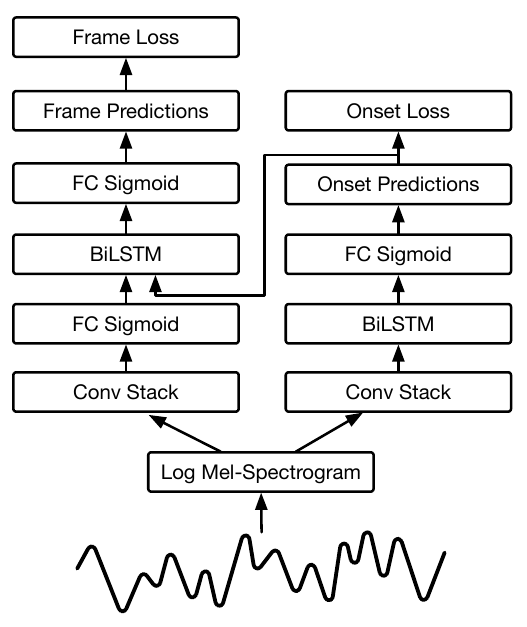
\includegraphics[height=8cm]{./statics/onset_onframe_architecture.png}
    \caption{ساختار شبکه استفاده شده در \cite{hawthorne2017onsets}}
\end{figure}

نکته قابل توجه این است که برای تشخیص شروع نت‌ها و فعال بودن نت‌ها از \gls{cnn} و
\gls{lstm} جداگانه استفاده شده است. دلیل استفاده از دو شبکه مجزا افزایش دقت نسبت
به حالت جایگزین هست. همچنین می‌توان شاهدی بر این باشد که هر بخش شبکه فقط اطلاعات
مورد نیاز برای هدف خود را یاد می‌گیرد.

در \cite{hawthorne2018enabling} نشان داده شد می‌توان از ساختار مشابه برای تشخیص
پایان نت‌ها نیز استفاده کرد. به این صورت که شبکه‌ای مشابه شبکه‌ تشخیص شروع نت
آموزش داده می‌شود. تابع خطایی که برای آموزش این شبکه استفاده می‌شود بر اساس
پایان نت‌ها ارزیابی را انجام می‌دهد. سپس در صورتی که این بخش شبکه پایان نتی را
پیشبینی کند، حتی اگه خروجی فعال بودن نت‌ها بگوید نت هنوز فعال است، نت پایان
یافته فرض می‌شود. به دلیل ساختار ساز پیانو وقتی که یک کلاویه راها می‌شود صدای
تولید شده بلافاصله قطع نمی‌شود و فقط مقداری از شدت آن کاسته می‌شود. داشتن یک
شبکه مجزا می‌توان به تشخیص این پایان‌ها کمک بسزایی کند و دقت را افزایش دهد.

یکی دیگر از نوآوری‌های \cite{hawthorne2017onsets} پیشبینی \gls{velocity} نت‌ها
در کنار پیشبینی \gls{pitch}، زمان شروع و زمان پایان نت‌هاست. \gls{velocity}
نت‌ها تاثیر بسزایی در درک ما از موسیقی و احساسی که در شونده القا می‌شود دارد.
\gls{velocity} بر خلاف مفاهیمی مانند \gls{pitch} یک مفهوم کاملا نسبی هست. به این
معنی که مقداری عددی برای اندازه‌گیری آن نمی‌توان استفاده کرد. دو نوازنده ممکن
است با قدرت‌های کاملا مختلفی یک قطعه را اجرا کنند ولی همچنان هر دو
\gls{velocity} مد نظر آهنگ‌ساز را به خوبی رعایت کرده باشند. برای حل این مشکل
ابتدا مقدار عددی متناظر در فایل‌های \gls{MIDI} تقسیم بر حداکثر \gls{velocity}
استفاده شده می‌شود. سپس از یک شبکه با ساختاری بسیار نزدیک به شبکه مسئول پیشبینی
onset استفاده می‌شود تا \gls{velocity} در نت را در زمان فعال شدن آن تخمین بزند.
این پیشبینی \glspl{velocity} باعث می‌شود که آوانویسی انجام شده توسط سیستم بسیار
طبیعی‌تر به نظر برسد و اجرای مجدد قطعه را بسیار ساده‌تر می‌کند.

\section{مقایسه روش‌های براساس فاکتورگیری نامنفی ماتریس و شبکه عصبی}
با توجه به محبوبیت \gls{nmf} و \gls{nn} برای حل مسئله \gls{atm} در ادامه به
بررسی تفاوت‌های این دو روش می‌پردازیم.

\gls{NMF} یک مدل خطی هست در حالی که \gls{NN} مدلی کاملا غیرخطی محسوب می‌شود.
اولین سوالی که مطرح می‌شود این هست که آیا این خطی بودن محدودیتی ایجاد خواهد کرد
یا نه. فرض کنید که به ازای هر \gls{pitch} دو قالب اسپکترال داریم. برای نمایش
\gls{spec} یک نت، دو قالب موجود را به صورت خطی با هم ترکیب می‌کنیم. ولی مجموعه
\gls{spec} متناظر با هر نت بسیار پیچیده‌تر هست و معمولا یک ترکیب خطی از آن‌ها
معادل یک ضبط واقعی نخواهد بود. می‌توانیم تعداد قالب‌های هر \gls{pitch} را افزایش
دهیم و مجددا تعداد نمایش‌ها نامعتر تولید شده بسیار بیشتر از نمایش‌ها معتبر خواهد
بود. از طرف دیگر \gls{nn} در سال‌های اخیر توانایی خوبی در نمایش این چنین
داده‌هایی را به صورت مقاوم و نسبت بهینه نشان داده‌اند \cite{goodfellow2016deep}.

یک مزیت دیگر مدل‌های برپایه \gls{NN} قابل آن‌ها برای آموزش به صورت \gls{e2e}
است. به این صورت که خروجی مدل می‌تواند مستقیم نت‌های تشخیص داده شده باشد و نیازی
به یک مرحله پس‌پردازش اضافه که در مدل‌های بر اساس \gls{NMF} لازم هست، نباشد.

با این وجود روش‌های مبتنی بر \gls{NMF} دو مزیت دارند که باعث می‌شود همچنان از
آن‌ها استفاده شود و نتایج قابل قبولی هم به دست آورند. مشکل اولی که در مقابل
\gls{nn} قرار دارد، کمبود دیتای مناسب هست. حتی بزرگ‌ترین \glspl{dataset} موجود
نیز در حد چند ساعت اطالاعت دارند. همچنین این دادگان از مشکل بایاس شدید رنج
می‌برند. شرایط ضبط هم معمولا تنوع لازم را ندارند و معمولا در چند محیط خاص و مدل
خاص ضبط انجام شده است. این محدودیت‌ها باعث می‌شود که همیشه خطر \gls{overfit}
وجود داشته باشد. همچنین برای بسیاری از سازها در لحظه هیچ \gls{dataset} وجود
ندارد.

مشکل دیگری که روش‌های مبتنی بر \gls{nn} از آن رنج می‌برند قابلیت تعمیم به شرایط
آکوستیکی جدید هست. معمولا مدل‌های برپایه \gls{nmf} موجود می‌تواند تنها با
استفاده از چند ثانیه از داده نواختن یک ساز جدید نتایج قابل قبولی بر ساز جدید
نمایش دهند. در لحظه هیچ شاهدی مبنی بر تونایی مشابه در روش‌های بر پایه \gls{NN}
ارائه نشده است. این دلیل باعث می‌شود که روش‌های مبتنی بر \gls{NMF} همچنان به
صورت گسترده مطالعه شوند و مورد استفاده قرار گیرند.